% Options for packages loaded elsewhere
% Options for packages loaded elsewhere
\PassOptionsToPackage{unicode}{hyperref}
\PassOptionsToPackage{hyphens}{url}
\PassOptionsToPackage{dvipsnames,svgnames,x11names}{xcolor}
%
\documentclass[
]{article}
\usepackage{xcolor}
\usepackage{amsmath,amssymb}
\setcounter{secnumdepth}{5}
\usepackage{iftex}
\ifPDFTeX
  \usepackage[T1]{fontenc}
  \usepackage[utf8]{inputenc}
  \usepackage{textcomp} % provide euro and other symbols
\else % if luatex or xetex
  \usepackage{unicode-math} % this also loads fontspec
  \defaultfontfeatures{Scale=MatchLowercase}
  \defaultfontfeatures[\rmfamily]{Ligatures=TeX,Scale=1}
\fi
\usepackage{lmodern}
\ifPDFTeX\else
  % xetex/luatex font selection
\fi
% Use upquote if available, for straight quotes in verbatim environments
\IfFileExists{upquote.sty}{\usepackage{upquote}}{}
\IfFileExists{microtype.sty}{% use microtype if available
  \usepackage[]{microtype}
  \UseMicrotypeSet[protrusion]{basicmath} % disable protrusion for tt fonts
}{}
\makeatletter
\@ifundefined{KOMAClassName}{% if non-KOMA class
  \IfFileExists{parskip.sty}{%
    \usepackage{parskip}
  }{% else
    \setlength{\parindent}{0pt}
    \setlength{\parskip}{6pt plus 2pt minus 1pt}}
}{% if KOMA class
  \KOMAoptions{parskip=half}}
\makeatother
% Make \paragraph and \subparagraph free-standing
\makeatletter
\ifx\paragraph\undefined\else
  \let\oldparagraph\paragraph
  \renewcommand{\paragraph}{
    \@ifstar
      \xxxParagraphStar
      \xxxParagraphNoStar
  }
  \newcommand{\xxxParagraphStar}[1]{\oldparagraph*{#1}\mbox{}}
  \newcommand{\xxxParagraphNoStar}[1]{\oldparagraph{#1}\mbox{}}
\fi
\ifx\subparagraph\undefined\else
  \let\oldsubparagraph\subparagraph
  \renewcommand{\subparagraph}{
    \@ifstar
      \xxxSubParagraphStar
      \xxxSubParagraphNoStar
  }
  \newcommand{\xxxSubParagraphStar}[1]{\oldsubparagraph*{#1}\mbox{}}
  \newcommand{\xxxSubParagraphNoStar}[1]{\oldsubparagraph{#1}\mbox{}}
\fi
\makeatother


\usepackage{longtable,booktabs,array}
\newcounter{none} % for unnumbered tables
\usepackage{calc} % for calculating minipage widths
% Correct order of tables after \paragraph or \subparagraph
\usepackage{etoolbox}
\makeatletter
\patchcmd\longtable{\par}{\if@noskipsec\mbox{}\fi\par}{}{}
\makeatother
% Allow footnotes in longtable head/foot
\IfFileExists{footnotehyper.sty}{\usepackage{footnotehyper}}{\usepackage{footnote}}
\makesavenoteenv{longtable}
\usepackage{graphicx}
\makeatletter
\newsavebox\pandoc@box
\newcommand*\pandocbounded[1]{% scales image to fit in text height/width
  \sbox\pandoc@box{#1}%
  \Gscale@div\@tempa{\textheight}{\dimexpr\ht\pandoc@box+\dp\pandoc@box\relax}%
  \Gscale@div\@tempb{\linewidth}{\wd\pandoc@box}%
  \ifdim\@tempb\p@<\@tempa\p@\let\@tempa\@tempb\fi% select the smaller of both
  \ifdim\@tempa\p@<\p@\scalebox{\@tempa}{\usebox\pandoc@box}%
  \else\usebox{\pandoc@box}%
  \fi%
}
% Set default figure placement to htbp
\def\fps@figure{htbp}
\makeatother


% definitions for citeproc citations
\NewDocumentCommand\citeproctext{}{}
\NewDocumentCommand\citeproc{mm}{%
  \begingroup\def\citeproctext{#2}\cite{#1}\endgroup}
\makeatletter
 % allow citations to break across lines
 \let\@cite@ofmt\@firstofone
 % avoid brackets around text for \cite:
 \def\@biblabel#1{}
 \def\@cite#1#2{{#1\if@tempswa , #2\fi}}
\makeatother
\newlength{\cslhangindent}
\setlength{\cslhangindent}{1.5em}
\newlength{\csllabelwidth}
\setlength{\csllabelwidth}{3em}
\newenvironment{CSLReferences}[2] % #1 hanging-indent, #2 entry-spacing
 {\begin{list}{}{%
  \setlength{\itemindent}{0pt}
  \setlength{\leftmargin}{0pt}
  \setlength{\parsep}{0pt}
  % turn on hanging indent if param 1 is 1
  \ifodd #1
   \setlength{\leftmargin}{\cslhangindent}
   \setlength{\itemindent}{-1\cslhangindent}
  \fi
  % set entry spacing
  \setlength{\itemsep}{#2\baselineskip}}}
 {\end{list}}
\usepackage{calc}
\newcommand{\CSLBlock}[1]{\hfill\break\parbox[t]{\linewidth}{\strut\ignorespaces#1\strut}}
\newcommand{\CSLLeftMargin}[1]{\parbox[t]{\csllabelwidth}{\strut#1\strut}}
\newcommand{\CSLRightInline}[1]{\parbox[t]{\linewidth - \csllabelwidth}{\strut#1\strut}}
\newcommand{\CSLIndent}[1]{\hspace{\cslhangindent}#1}



\setlength{\emergencystretch}{3em} % prevent overfull lines

\providecommand{\tightlist}{%
  \setlength{\itemsep}{0pt}\setlength{\parskip}{0pt}}



 


\makeatletter
\@ifpackageloaded{caption}{}{\usepackage{caption}}
\AtBeginDocument{%
\ifdefined\contentsname
  \renewcommand*\contentsname{Table of contents}
\else
  \newcommand\contentsname{Table of contents}
\fi
\ifdefined\listfigurename
  \renewcommand*\listfigurename{List of Figures}
\else
  \newcommand\listfigurename{List of Figures}
\fi
\ifdefined\listtablename
  \renewcommand*\listtablename{List of Tables}
\else
  \newcommand\listtablename{List of Tables}
\fi
\ifdefined\figurename
  \renewcommand*\figurename{Figure}
\else
  \newcommand\figurename{Figure}
\fi
\ifdefined\tablename
  \renewcommand*\tablename{Table}
\else
  \newcommand\tablename{Table}
\fi
}
\@ifpackageloaded{float}{}{\usepackage{float}}
\floatstyle{ruled}
\@ifundefined{c@chapter}{\newfloat{codelisting}{h}{lop}}{\newfloat{codelisting}{h}{lop}[chapter]}
\floatname{codelisting}{Listing}
\newcommand*\listoflistings{\listof{codelisting}{List of Listings}}
\makeatother
\makeatletter
\makeatother
\makeatletter
\@ifpackageloaded{caption}{}{\usepackage{caption}}
\@ifpackageloaded{subcaption}{}{\usepackage{subcaption}}
\makeatother
\usepackage{bookmark}
\IfFileExists{xurl.sty}{\usepackage{xurl}}{} % add URL line breaks if available
\urlstyle{same}
% fallback for those not using the hyperref driver hyperxmp:
\makeatletter
\@ifundefined{xmpquote}{\newcommand{\xmpquote}[1]{#1}}{}
\makeatother
\hypersetup{
  pdftitle={Is everything a Niche model? Food Web Reconstruction Frameworks Converge in Structure but Diverge in {[}something{]}},
  pdfauthor={Tanya Strydom; Xiaoxiao Li; Laura Sophia Landon Blake; Andrew P. Beckerman; Dylan Z. Childs},
  pdfkeywords={\xmpquote{food web
reconstruction}, \xmpquote{bioenergetic dynamics}, \xmpquote{network
stability}, \xmpquote{ecological networks}, \xmpquote{generative
models}, \xmpquote{community persistence}},
  colorlinks=true,
  linkcolor={blue},
  filecolor={Maroon},
  citecolor={Blue},
  urlcolor={Blue},
  pdfcreator={LaTeX via pandoc}}



\title{Is everything a Niche model? Food Web Reconstruction Frameworks
Converge in Structure but Diverge in {[}something{]}}
\author{Tanya Strydom %
%
\textsuperscript{%
%
1%
}%
; Xiaoxiao Li %
%
\textsuperscript{%
%
1%
}%
; Laura Sophia Landon Blake %
%
\textsuperscript{%
%
1%
}%
; Andrew P. Beckerman %
%
\textsuperscript{%
%
1%
}%
; Dylan Z. Childs %
%
\textsuperscript{%
%
1%
}%
}
\date{2026-09-04}

\usepackage{setspace}
\usepackage[left]{lineno}
\usepackage[letterpaper]{geometry}

\usepackage[nolists,noheads,markers]{endfloat}
\geometry{margin=2.5cm}

\begin{document}

\thispagestyle{empty}
{\bfseries\sffamily\Large Is everything a Niche model? Food Web
Reconstruction Frameworks Converge in Structure but Diverge in
{[}something{]}}
\vfil
Tanya Strydom %
%
\textsuperscript{%
%
1%
}%
; Xiaoxiao Li %
%
\textsuperscript{%
%
1%
}%
; Laura Sophia Landon Blake %
%
\textsuperscript{%
%
1%
}%
; Andrew P. Beckerman %
%
\textsuperscript{%
%
1%
}%
; Dylan Z. Childs %
%
\textsuperscript{%
%
1%
}%

\vfil
{\small
\textbf{Abstract:} Food web ecology relies heavily on generative models
to reconstruct trophic interactions, yet these models embody
fundamentally different assumptions about how ecological communities are
assembled. Whether these alternative reconstruction frameworks provide
interchangeable baselines for studying ecosystem dynamics remains
largely unknown. Here, we compared seven food web generative models
spanning structural, statistical, and trait-based approaches by
embedding each within an identical bioenergetic simulation framework
while controlling species pools and dynamical rules. Initial networks
generated by different frameworks occupied distinct regions of
multivariate topology space, demonstrating that reconstruction framework
alone produces substantially different food web architectures. Following
bioenergetic simulations, however, realised networks converged towards a
shared region of topology space through extinction-driven pruning of
species and interactions, indicating that ecological dynamics impose
strong constraints on viable network structure. Despite this structural
convergence, predictions of biomass equilibrium did not converge. Local
stability metrics, including resilience and reactivity, remained
strongly dependent on the original generative model, whereas broader
network-level properties were explained primarily by realised species
richness rather than reconstruction framework. Our results reveal a
decoupling between structural and dynamical convergence. Ecological
dynamics filter diverse initial architectures towards persistent network
structures, but they retain the historical signature of the assumptions
used to reconstruct trophic interactions. This suggests that generative
models are not interchangeable starting points for ecological inference.
Structural models provide useful approximations for broad topological
and diversity patterns, whereas trait-based models are required to
capture transient dynamics and local stability. Rather than treating
food web reconstruction as a universal modelling baseline,
reconstruction frameworks should be chosen according to the ecological
questions they are intended to answer.
\vfil
\textbf{Keywords:} %
food web reconstruction, bioenergetic dynamics, network
stability, ecological networks, generative models, %
community persistence%
}
\clearpage
\setcounter{page}{1}
\doublespacing
\linenumbers


\section{Introduction}\label{introduction}

For over two decades, community ecology has relied heavily on generative
models to understand and reconstruct the structure of trophic networks.
At the centre of this framework is the niche model. Introduced by
Williams \& Martinez (2000) as a major advance over the strictly
hierarchical Cascade model (Cohen et al., 1990), the Niche model
demonstrated that relatively simple assembly rules could reproduce many
emergent properties of empirical food webs, including realistic degree
distributions, trophic guild proportions, and path lengths. This success
has established the niche model as the default structural baseline for
investigating macroecological patterns, robustness to primary
extinctions, and the stability of ecological communities (Allesina \&
Tang, 2012; Curtsdotter et al., 2011).

The widespread use of the Niche model has also encouraged a broader
assumption that different food web reconstruction methods provide
interchangeable representations of ecological communities. However,
generative models embody fundamentally different assumptions about how
trophic interactions arise (Strydom, Dunhill, et al., 2026). Structural
models operate from the network down, generating interactions according
to statistical or topological rules. The Niche and Cascade models impose
ordered feeding hierarchies along a latent niche axis, while maximum
entropy (MaxEnt) models generate networks that satisfy macroscopic
constraints while remaining maximally unstructured beyond those
constraints (Banville et al., 2023). In contrast, mechanistic approaches
operate from the species up, constructing networks from organismal
traits and ecological processes. The Allometric Diet Breadth Model
(ADBM) derives realised diets from optimal foraging and energetic
profitability(Petchey et al., 2008), whereas the Allometric Trophic
Network (ATN) framework constrains interactions through body-size
scaling and metabolic theory (Brose et al., 2006; Schneider et al.,
2016). Latent trait models occupy an intermediate position, inferring
interactions statistically from underlying species traits without
prescribing explicit feeding rules (Rohr et al., 2010).

These contrasting modelling philosophies raise a fundamental question.
Are they simply different routes to the same ecological inference, or do
they encode different assumptions about network architecture that
persist into predictions of ecosystem dynamics? Recent work has shown
that applying different reconstruction frameworks to identical species
pools produces markedly different food web topologies and inference
about species extinctions (Strydom, Karapunar, et al., 2026). Because
network architecture governs the pathways through which energy, biomass,
and indirect effects propagate through communities (Delmas et al.,
n.d.), differences in reconstruction may have important consequences for
ecological dynamics rather than representing alternative but equivalent
descriptions of the same system.

At the same time, empirical food webs exhibit surprisingly consistent
local structural organisation despite large differences in species
composition and ecosystem type, suggesting that ecological communities
occupy a constrained region of possible network architectures rather
than arbitrary combinations of interactions. This has motivated the idea
that ecological dynamics selectively retain interaction structures that
are compatible with persistence while filtering those that are not
(Stouffer et al., 2007; Stouffer \& Bascompte, 2010). Whether this
filtering is sufficiently strong to erase the structural differences
introduced by alternative reconstruction frameworks remains unknown.

Here, we test whether food web reconstruction frameworks function as
benign structural templates or whether they fundamentally shape
ecological inference. We generated food webs using seven models spanning
structural, statistical, and trait-based philosophies and embedded each
within an identical bioenergetic simulation framework while controlling
species pools and dynamical rules. This design allows us to separate the
effects of network construction from the effects of ecological dynamics
and ask two questions: (i) do different reconstruction frameworks
converge towards a common realised network structure under bioenergetic
dynamics, and (ii) if structural convergence occurs, do predictions of
biomass equilibrium also converge, or do they retain a signature of the
original generative model?

\section{Methods}\label{methods}

\subsection{Network generation}\label{network-generation}

We generated food webs using six established generative models, spanning
structural (Niche, Cascade, Random, MaxEnt) and trait-based approaches
(Latent Trait Model, Allometric Trophic Network, Allometric Diet Breadth
Model), see Table~\ref{tbl-models} for more details. All simulations
were implemented in Julia (Bezanson et al., 2017) and analyses in R (R
Core Team, 2024).

\begin{longtable}[]{@{}
  >{\raggedright\arraybackslash}p{(\linewidth - 6\tabcolsep) * \real{0.2466}}
  >{\raggedright\arraybackslash}p{(\linewidth - 6\tabcolsep) * \real{0.2466}}
  >{\raggedright\arraybackslash}p{(\linewidth - 6\tabcolsep) * \real{0.2466}}
  >{\raggedright\arraybackslash}p{(\linewidth - 6\tabcolsep) * \real{0.2603}}@{}}
\caption{Summary of food web models used in this study. Structural
models (Niche, Cascade, MaxEnt) generate network topology based on
abstract or statistical rules, while realised/dynamic models (ADBM, ATN,
Latent trait) incorporate species-specific traits and biological
mechanisms to predict interactions. For each model, we list the main
inputs and the key assumptions that govern link
formation.}\label{tbl-models}\tabularnewline
\toprule\noalign{}
\begin{minipage}[b]{\linewidth}\raggedright
Model
\end{minipage} & \begin{minipage}[b]{\linewidth}\raggedright
Type
\end{minipage} & \begin{minipage}[b]{\linewidth}\raggedright
Main Inputs
\end{minipage} & \begin{minipage}[b]{\linewidth}\raggedright
Key Assumptions
\end{minipage} \\
\midrule\noalign{}
\endfirsthead
\toprule\noalign{}
\begin{minipage}[b]{\linewidth}\raggedright
Model
\end{minipage} & \begin{minipage}[b]{\linewidth}\raggedright
Type
\end{minipage} & \begin{minipage}[b]{\linewidth}\raggedright
Main Inputs
\end{minipage} & \begin{minipage}[b]{\linewidth}\raggedright
Key Assumptions
\end{minipage} \\
\midrule\noalign{}
\endhead
\bottomrule\noalign{}
\endlastfoot
Niche model (Williams \& Martinez, 2000) & Structural & Species niche
values & Trophic interactions structured by a one-dimensional feeding
niche; species consume all prey within a contiguous range; allows
cannibalism. \\
Cascade model (Cohen et al., 1990) & Structural & Species rank &
Consumers feed only on species with lower ranks; strictly hierarchical;
no loops or omnivory. \\
MaxEnt model (Banville et al., 2023) & Structural & Species richness,
connectance & Links assigned to maximise entropy; captures global
network properties without species-specific mechanisms. \\
Allometric Diet Breadth Model (ADBM) (Petchey et al., 2008) & Realised &
Body mass, prey energy content & Consumers maximize energy intake; diet
breadth determined by profitability and handling time; allometric
scaling governs parameters. \\
Allometric Trophic Network (ATN) (Brose et al., 2006) & Realised & Body
mass & Interactions constrained by body mass ratios; mechanical size
limits structure networks; probability of interaction follows Ricker
function. \\
Latent trait model (Rohr et al., 2010) & Realised & Species traits
(\emph{e.g.,} body mass) & Interactions inferred statistically based on
hidden trait correlations; can incorporate probabilistic constraints on
links. \\
\end{longtable}

To isolate model effects from input variation, all trait-based models
were parameterised using an identical species pool at each replicate.
Species richness was set to 10, 20, 40, and for each iteration we
sampled (i) a target basal fraction (U(0.1,0.3)), (ii) metabolic classes
consistent with this fraction, and (iii) body masses from class-specific
log-uniform distributions. These inputs were shared across the Latent
Trait, ATN, and ADBM models. Structural models were instead
parameterised by a target connectance drawn from U(0.05, 0.3) where
relevant. This allows one to isolate the effect of network-generating
assumptions by holding constant (i) species richness, (ii) trait
distributions (within trait-based models), and (iii) dynamical rules.
Differences in structure and dynamics can therefore be attributed
directly to the generative model used to reconstruct trophic
interactions.

Networks were generated using a rejection-sampling procedure to enforce
comparable emergent properties. A network was retained only if its
realised basal fraction and connectance fell within the target ranges
(0.1--0.3 and 0.05--0.3, respectively). For trait-based models, networks
were accepted only when all three models successfully generated valid
networks from the same species pool. We obtained \textbf{100} valid
replicates per model, with an upper bound on sampling attempts to
prevent non-termination. MaxEnt networks were constructed by sampling
joint in- and out-degree distributions consistent with a target number
of links, followed by entropy-maximising rewiring under degree
constraints. The Niche and Cascade networks were constructed using the
target connectance and species richness.

\subsection{Network structure}\label{network-structure}

All networks were converted to directed interaction networks and
analysed using a standardised pipeline. We quantified structural
properties across multiple scales, including connectance, trophic level,
generality, vulnerability, clustering, centrality, trophic coherence,
and path length. These metrics were used to characterise the structural
signature of each model.

\begin{quote}
I can do a supp matt that breaks all the structural metrics down - I
don't think we need it here in the main text.
\end{quote}

\subsection{Dynamic simulations}\label{dynamic-simulations}

To evaluate the dynamical consequences of different generative models,
we simulated each network using the bio-energetic food web dynamic model
implemented in \texttt{EcologicalNetworksDynamics.jl} (Lajaaiti et al.,
2025). A key feature of the bio-energetic model is the allometric
scaling of metabolism, growth and foraging rates with body mass. For
trait-based models (ATN, ADBM, LTN), species body masses were taken from
the generative networks and rescaled relative to the producer with the
lowest body mass. For structural models (Niche, Cascade, MaxEnt,
Random), which did not include body mass information, body masses were
assigned from species trophic levels assuming apredator--prey body mass
ratio of 100.

For a consumer species \(i\), biomass dynamics were determined by gains
from feeding, losses to predators, and metabolic maintenance, which is
expressed as:

\[
\frac{dB_i}{dt} = \sum_{j \in \mathrm{prey}(i)}e_{ij} B_i F_{ij} - \sum_{j \in \mathrm{predators}(i)} B_j F_{ji} - x_i B_i
\]

where \(B_i\) is the biomass of consumer \(i\), \(e_{ij}\) is its
assimilation efficiency when feeding on prey \emph{j}, \(x_i\) is its
metabolic rate scaled with body mass, and \(F_{ij}\) is the functional
response of consumer \emph{i} feeding on prey \emph{j}, defined as

\[
F_{ij} = \frac{\omega_{i} a_{ij} B_j^{h}} {M_i\left (1 + \displaystyle\sum_{k \in \mathrm{prey}(i)} \omega_{i} a_{ik} h_{ik} B_k^{h} \right)}
\]

where \(w_i\) is the equal preference of the consumer i feeding on its
prey, \(w_i\) = 1/number of prey species. \(a_{ij}\) is the attack rate,
\(h_{ij}\) is the handling time, and \(M_i\) is the body mass of
consumer \emph{i}. Attack rates and handling times scaled with both
consumer and prey body masses. The Hill exponent was set to \(h = 2\) as
a Type III functional response.

For a basal species \(j\), biomass dynamics were determined by its
logistic growth and losses to consumers, expressed as:

\[
\frac{dB_j}{dt} = r_j G_j B_j - \sum_{i \in \mathrm{predators}(j)} B_i F_{ij}
\]

where \(r_j\) is the intrinsic growth rate and
\(G_j = 1 - \frac{B_j}{K_j}\) is the logistic growth modifier , with
\(K_j\) is the carrying capacity. Both \(r_j\) and \(K_j\) scaled with
species body mass.

All allometric constants used to parametrise \(x_i\), \(a_{ij}\),
\(h_{ij}\), \(r_j\), and \(K_j\) were set to the default values provided
by (Lajaaiti et al., 2025).

Each network was simulated until it reached a steady state. Species were
considered extinct when their biomass fell below \(10^{−6}\). At
equilibrium, both extinct species and disconnected species were removed,
yielding the realised post-simulation network.

\subsection{Post-simulation analyses}\label{post-simulation-analyses}

\subsubsection{Phenotypic trajectory
analysis}\label{phenotypic-trajectory-analysis}

To quantify how ecological dynamics reshaped network topology, all
structural metrics were recalculated following the dynamic simulations
using the realised (post-extinction) network. These post-dynamics
metrics were compared with those of the initial network using a
phenotypic trajectory analysis (PTA) framework (Adams \& Collyer, 2009),
where each network was represented as a point in a multivariate topology
space defined by the suite of structural network metrics {[}TABLE in
SI{]}. Prior to analysis, all metrics were standardised (mean = 0, SD =
1) to remove differences in scale before constructing a common topology
space using principal component analysis (PCA). Both pre- and
post-dynamics networks were projected into this shared ordination,
allowing each network to be represented by a trajectory from its initial
to realised topology.

Trajectory vectors were calculated as the displacement between pre- and
post-dynamics positions in the five-dimensional PCA space. Trajectory
length was calculated as the Euclidean distance between the two states,
providing a measure of the magnitude of topological change. Mean
trajectories were calculated for each network reconstruction model
centroid to summarise their overall direction of change. Finally,
convergence among network topologies was assessed by calculating each
network's Euclidean distance to the global post-dynamics centroid before
and after simulation, with positive reductions in distance indicating
convergence towards a common realised network topology.

\subsubsection{Community stability}\label{community-stability}

At equilibrium, we calculated two sets of stability metrics to compare
realised networks across generative models. First, network-level
stability was characterised by species persistence, Shannon diversity of
biomasses, the Gini coefficient of consumption fluxes, and the skewness
of interspecific interaction strengths. Second, local stability was
characterised by resilience and reactivity. Resilience was measured by
the real part of the dominant eigenvalue of the Jacobian matrix, with
more negative values indicating faster return to equilibrium following a
small perturbation (Ruiter et al., 1995). Reactivity quantified the
maximum instantaneous amplification of perturbations, with more positive
values indicating a stronger tendency for some perturbations to
initially move the system further away from equilibrium (Neubert \&
Caswell, 1997).

For each stability metric, we fitted a linear model including food web
model and equilibrium species richness as additive predictors:

\(\text{Stability metric} \sim \text{Food web model} + \text{Equilibrium richness}\).

We used Type II ANOVA to assess the contribution of each predictor while
controlling for the other. The magnitude of each association was
quantified using partial eta-squared, which represents the proportion of
effect-plus-residual variation attributable to a predictor after
accounting for the other predictor.

\section{Results}\label{results}

\subsection{Networks Converge in
Structure}\label{networks-converge-in-structure}

Projection of all networks into a common topology space revealed that
initial and realised food web topologies occupied distinct regions of
multivariate space (Figure~\ref{fig-PTA} A). The first two principal
components explained 50.7\% of the total variation in network structure,
with variation primarily associated with linkage density, chain length,
and direct competition (S4) (Figure~\ref{fig-PTA} B). While considerable
separation among reconstruction models was evident in the initial
topology space, post-dynamics networks exhibited greater overlap,
suggesting that ecological dynamics altered structural differences among
models.

\begin{figure}

\centering{

\pandocbounded{\includegraphics[keepaspectratio]{figures/PTA.png}}

}

\caption{\label{fig-PTA}Ecological dynamics reshape food web topology
within a shared multivariate topology space. Network structural metrics
were standardised and summarised using principal component analysis,
with each network represented by its position before and after dynamic
simulations. (A) PCA of networks before and after dynamic simulations.
Ellipses cover 90\% of points (B) Principal component loadings showing
the contribution of the top ten individual network metrics to topology
space (C) Centroid trajectories for each reconstruction model,
illustrating the direction and magnitude of topological change between
initial and realised networks. (D) Displacement of model centroids as
trajectory lengths over the first five principal component axes, points
represent mean length (E) Mean Euclidean distance of networks to the
centroid before and after simulations, providing a measure of
convergence in network topology.}

\end{figure}%

All reconstruction models underwent measurable shifts in topology
following dynamic simulations, although both the magnitude and direction
of change differed among models (Figure~\ref{fig-PTA} C). Centroid
trajectories showed that all models moved broadly in the same direction,
indicating that ecological dynamics reshaped network topology in a
consistent manner. This can be seen when looking at the displacement of
models along the various PC axes (Figure~\ref{fig-PTA} D), where all
models showed the greatest displacement along PC1.

Finally, realised networks showed evidence of convergence within
topology space (Figure~\ref{fig-PTA} E). The mean Euclidean distance to
the global realised-network centroid decreased following dynamic
simulations for all models, suggesting that ecological dynamics drove
networks towards a common structural endpoint despite differences in
initial topology.

\subsection{Structure does not confer
stability}\label{structure-does-not-confer-stability}

With the exception of the Niche and Cascade models not all networks
reached an equilibrium biomass (Figure~\ref{fig-stability_endpnts}). The
Random networks had the lowest percentage of networks that reached an
equilibrium state, with most of the networks collapsing \emph{i.e.,}
species went extinct. With the two structural networks (Random and
MaxEnt) we see that the larger the initial network is the more of them
fail to reach an equilibrium state. Conversely the three body size
models (ADBM, ATN, and LTM) show the opposite relationship (smaller
networks tend to fail). Interestingly we primarily see that networks
fail due to extinction of the community as opposed to the network not
being able to reach an equilibrium state.

\begin{figure}

\centering{

\pandocbounded{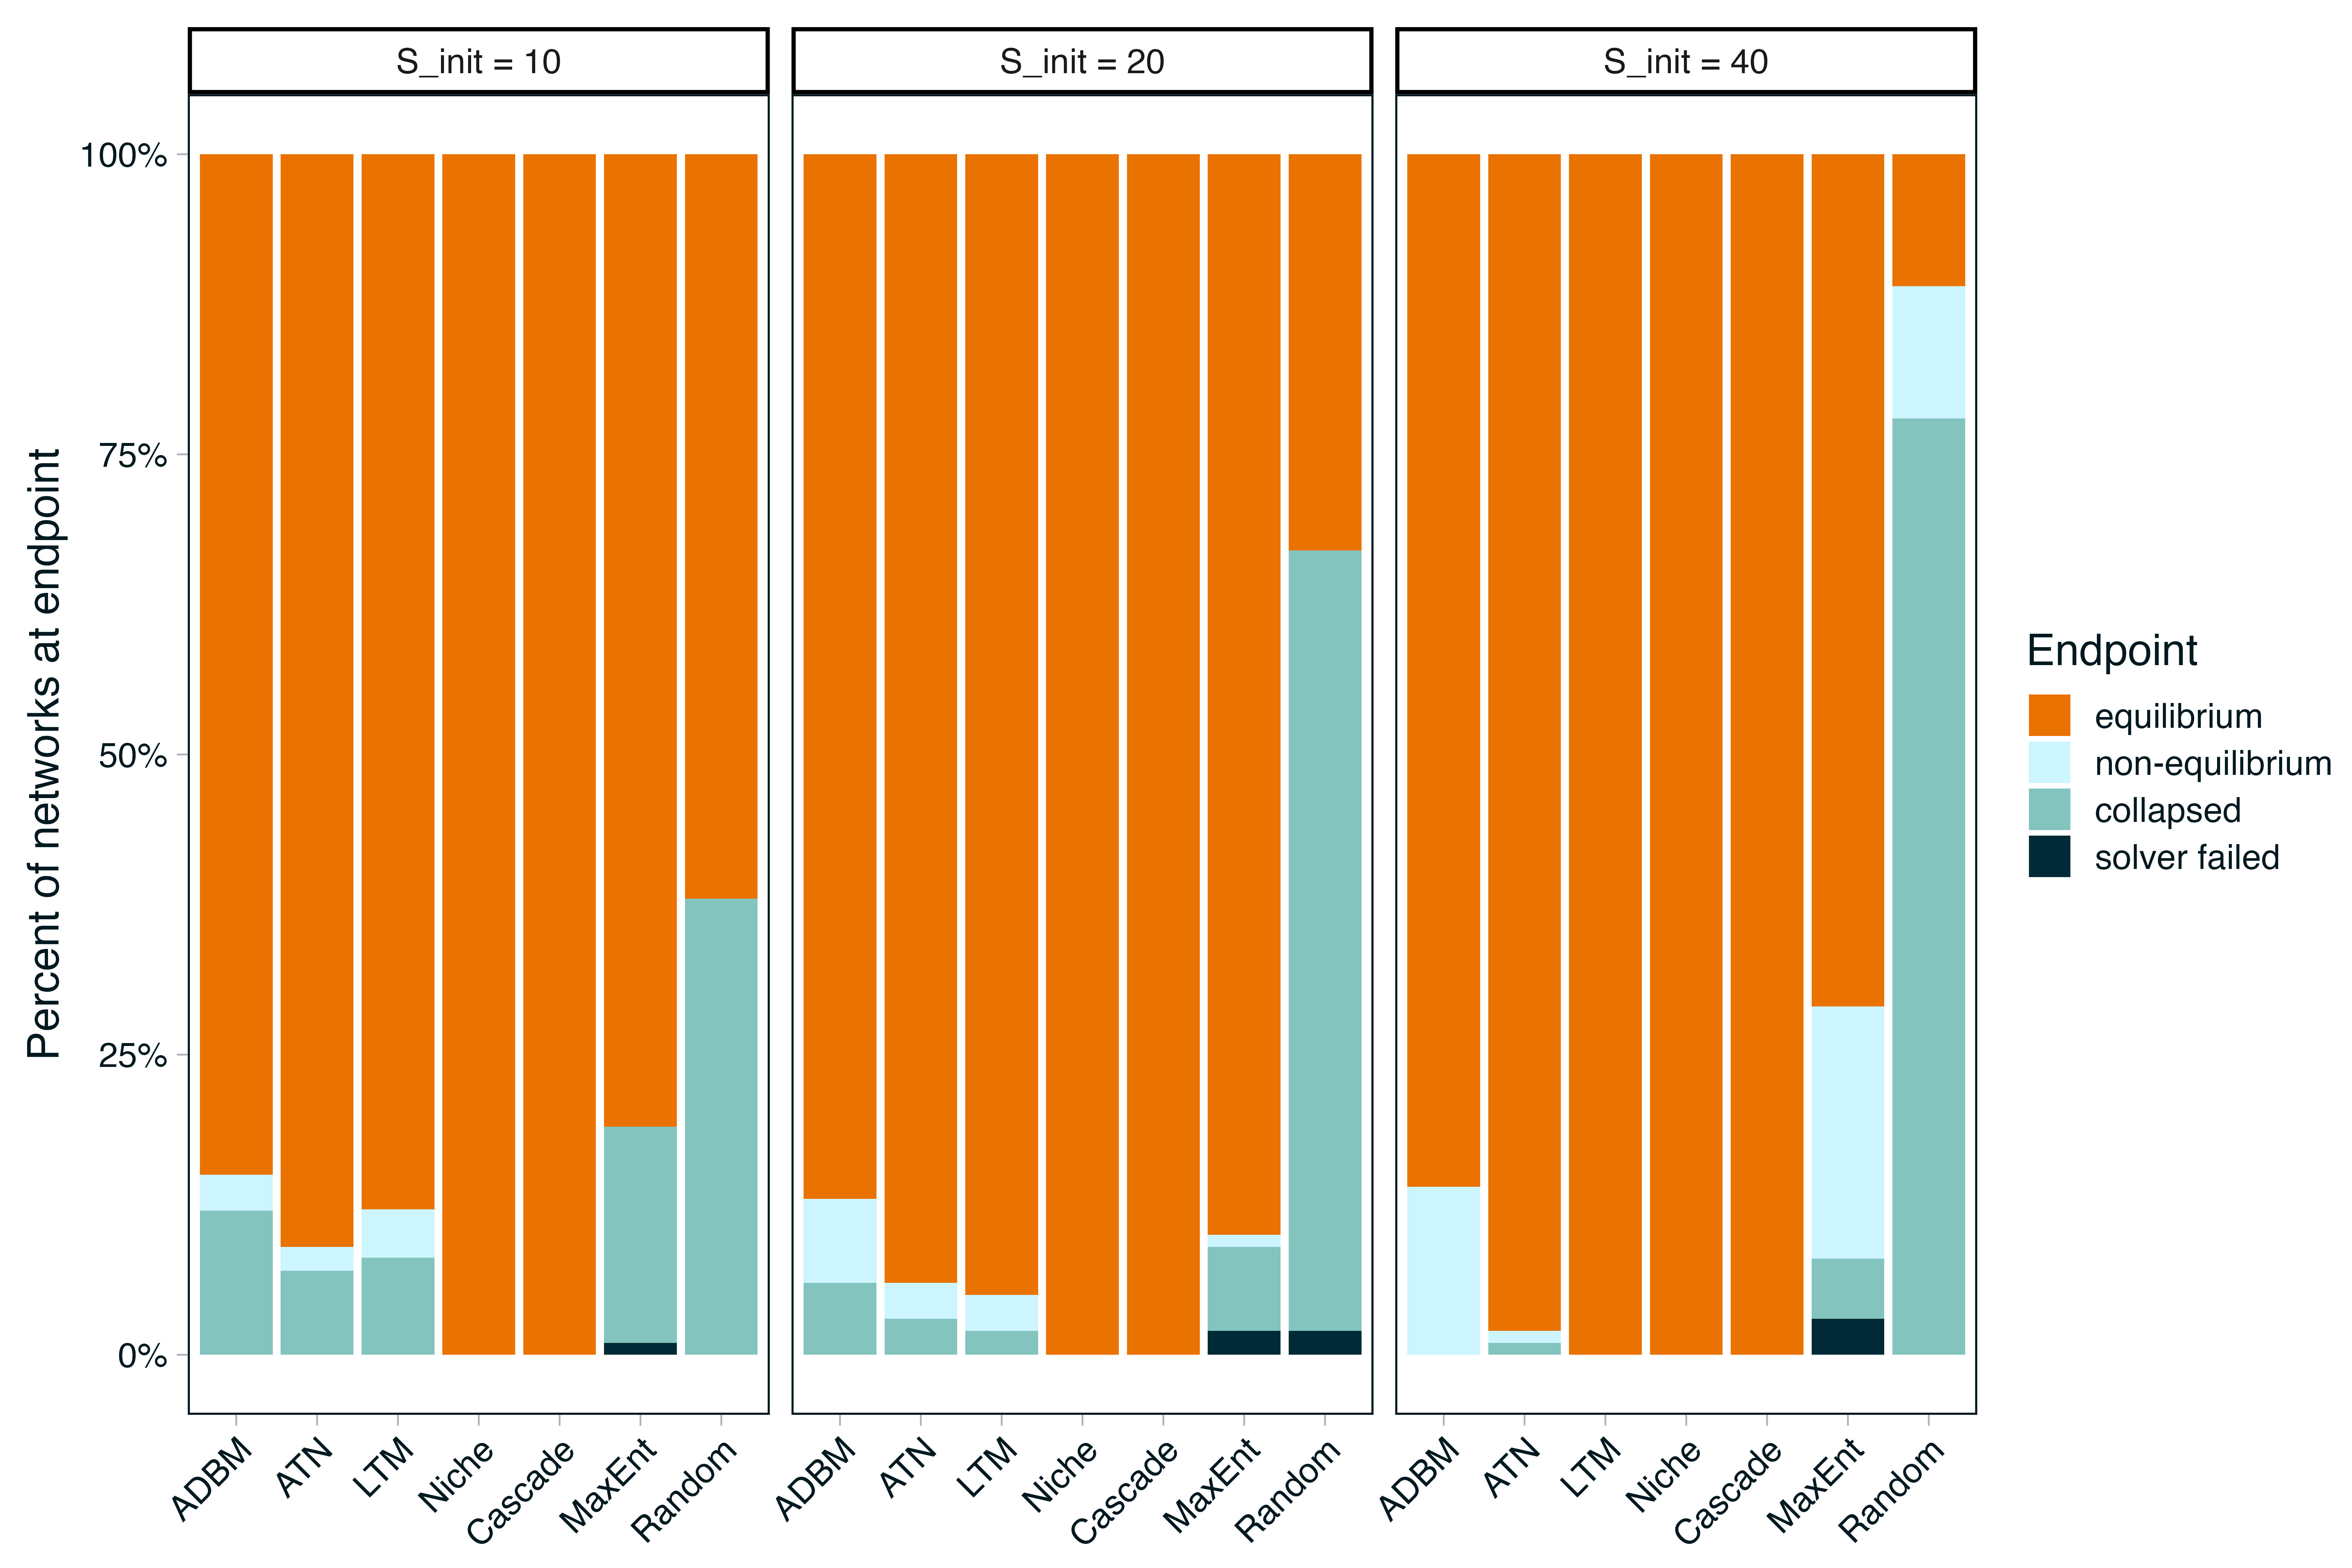
\includegraphics[keepaspectratio]{figures/stability_endpoints.png}}

}

\caption{\label{fig-stability_endpnts}End points of networks indicating
the percentage of networks that reached an equilibrium biomass (orange)
and if they did not (shades of blue) why not. These are faceted by the
initial starting richness for each network}

\end{figure}%

Interestingly if we plot the `failed' networks into the PCA space
(Figure~\ref{fig-failed_pca}, darker points) these networks do not
differ obviously in structure with the `successful' networks. What is
perhaps notable though is that we do begin to see some deviation in this
observation for the larger networks (right column,
Figure~\ref{fig-failed_pca}), with these networks typically being on the
`end range' of the pre structural space.

\begin{figure}

\centering{

\pandocbounded{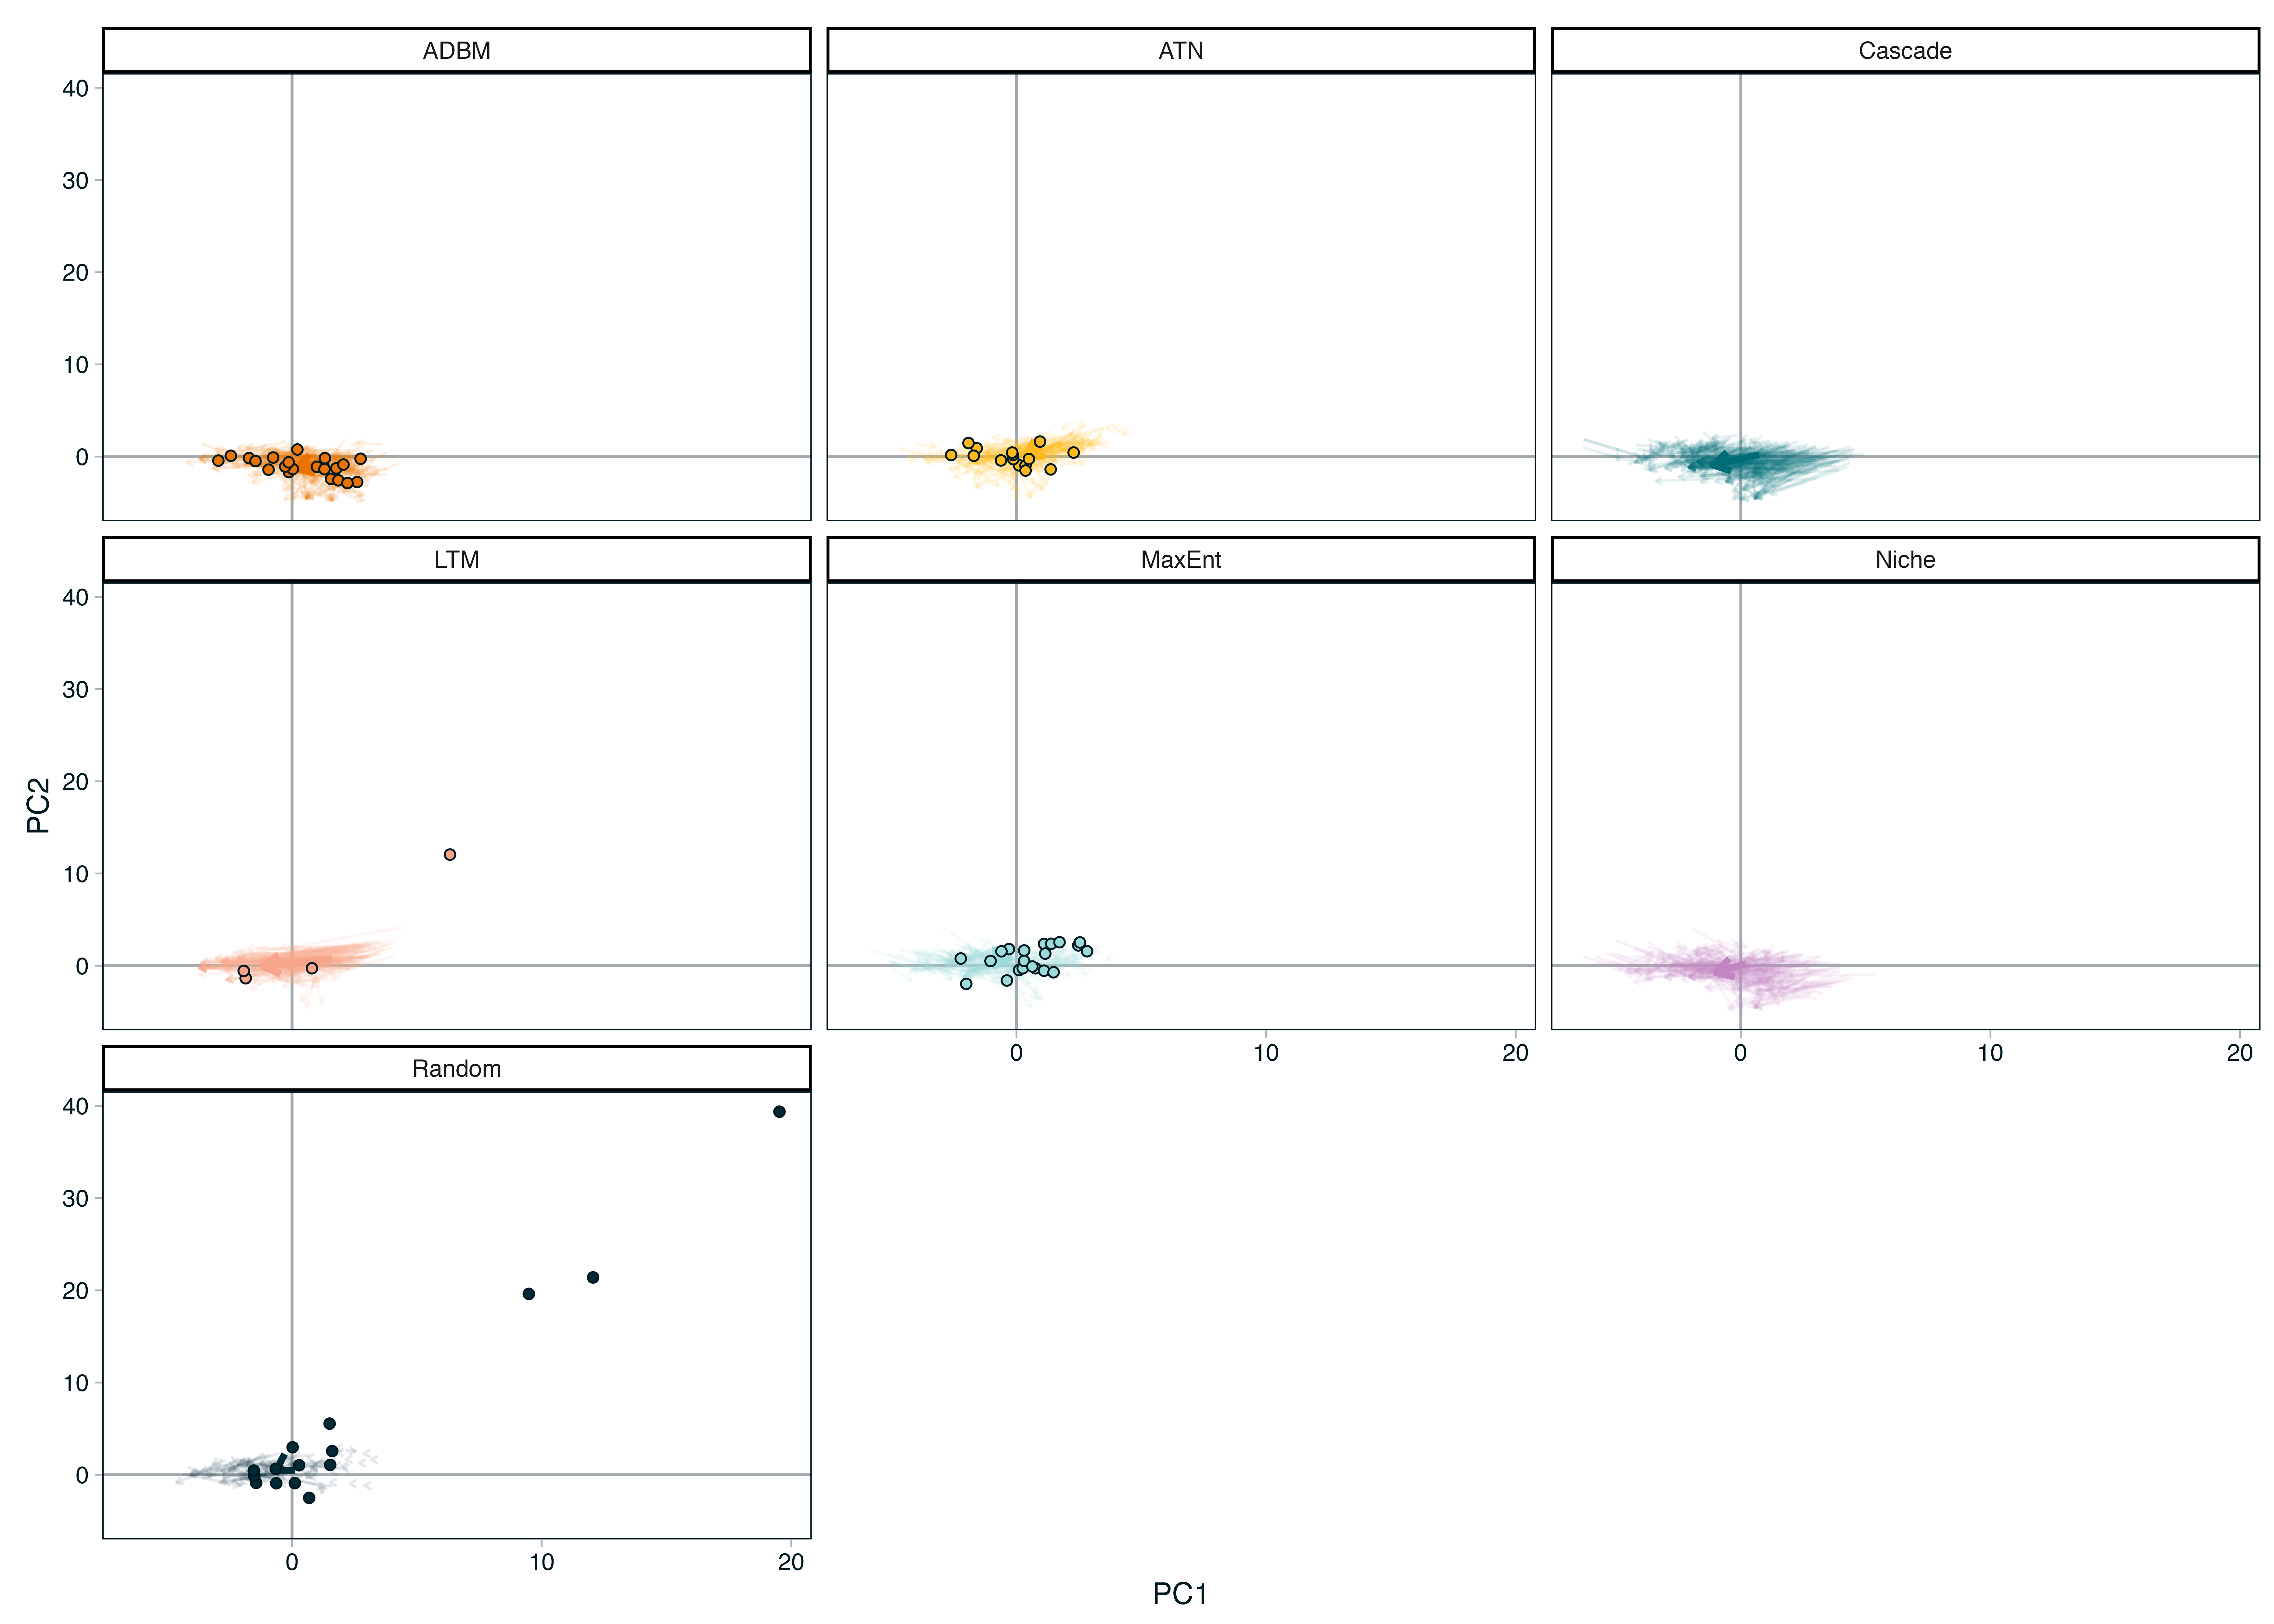
\includegraphics[keepaspectratio]{figures/PTA_failed_networks.png}}

}

\caption{\label{fig-failed_pca}Arrows indicate trajectory of individual
networks. Points are networks that failed to reach an equilibrium state
that have been predicted into the PCA space. Pale arrows show the
trajectory of each individual network, dark arrows the mean trajectory.
Note we do not plot networks that failed due to solver issues,
additionally we omit the Niche and Cascade models as they have no failed
networks}

\end{figure}%

\subsection{Network stability
inferences}\label{network-stability-inferences}

Equilibrium richness explained substantially more variation than
generative food web models in network-level stability metrics, with the
strongest contribution observed for Shannon diversity of biomasses,
followed by the skewness of interaction strengths, species persistence
and the Gini coefficient of consumption fluxes
(Figure~\ref{fig-rel_contribution}). In contrast, variation in
resilience was influenced by both richness and model, with a larger
contribution from model. Reactivity was explained primarily by
generative food web models, with very little contribution from
equilibrium richness.

\begin{figure}

\centering{

\pandocbounded{
\includegraphics[keepaspectratio]{figures/stability_effect_size_model_vs_richness.png}}

}

\caption{\label{fig-rel_contribution}Relative contributions of
equilibrium species richness and generative food web models to variation
in network and local stability metrics}

\end{figure}%

After accounting for equilibrium richness, Niche, Cascade, ATN and
MaxEnt generally supported higher species persistence than ADBM, LTM and
Random generated food webs (Figure~\ref{fig-emmeans}). Biomass diversity
was highest in Cascade and Niche webs, but comparatively low in LTM and
MaxEnt. Random model had the most uneven consumption fluxes, while
MaxEnt and Random webs showed the strongest skewness in interaction
strengths. ADBM and LTM generated food webs showed the highest
resilience, i.e.,fastest asymptotic recovery, whereas LTM food webs were
also the most reactive, i.e., strongest initial amplification of
perturbations.

\begin{figure}

\centering{

\pandocbounded{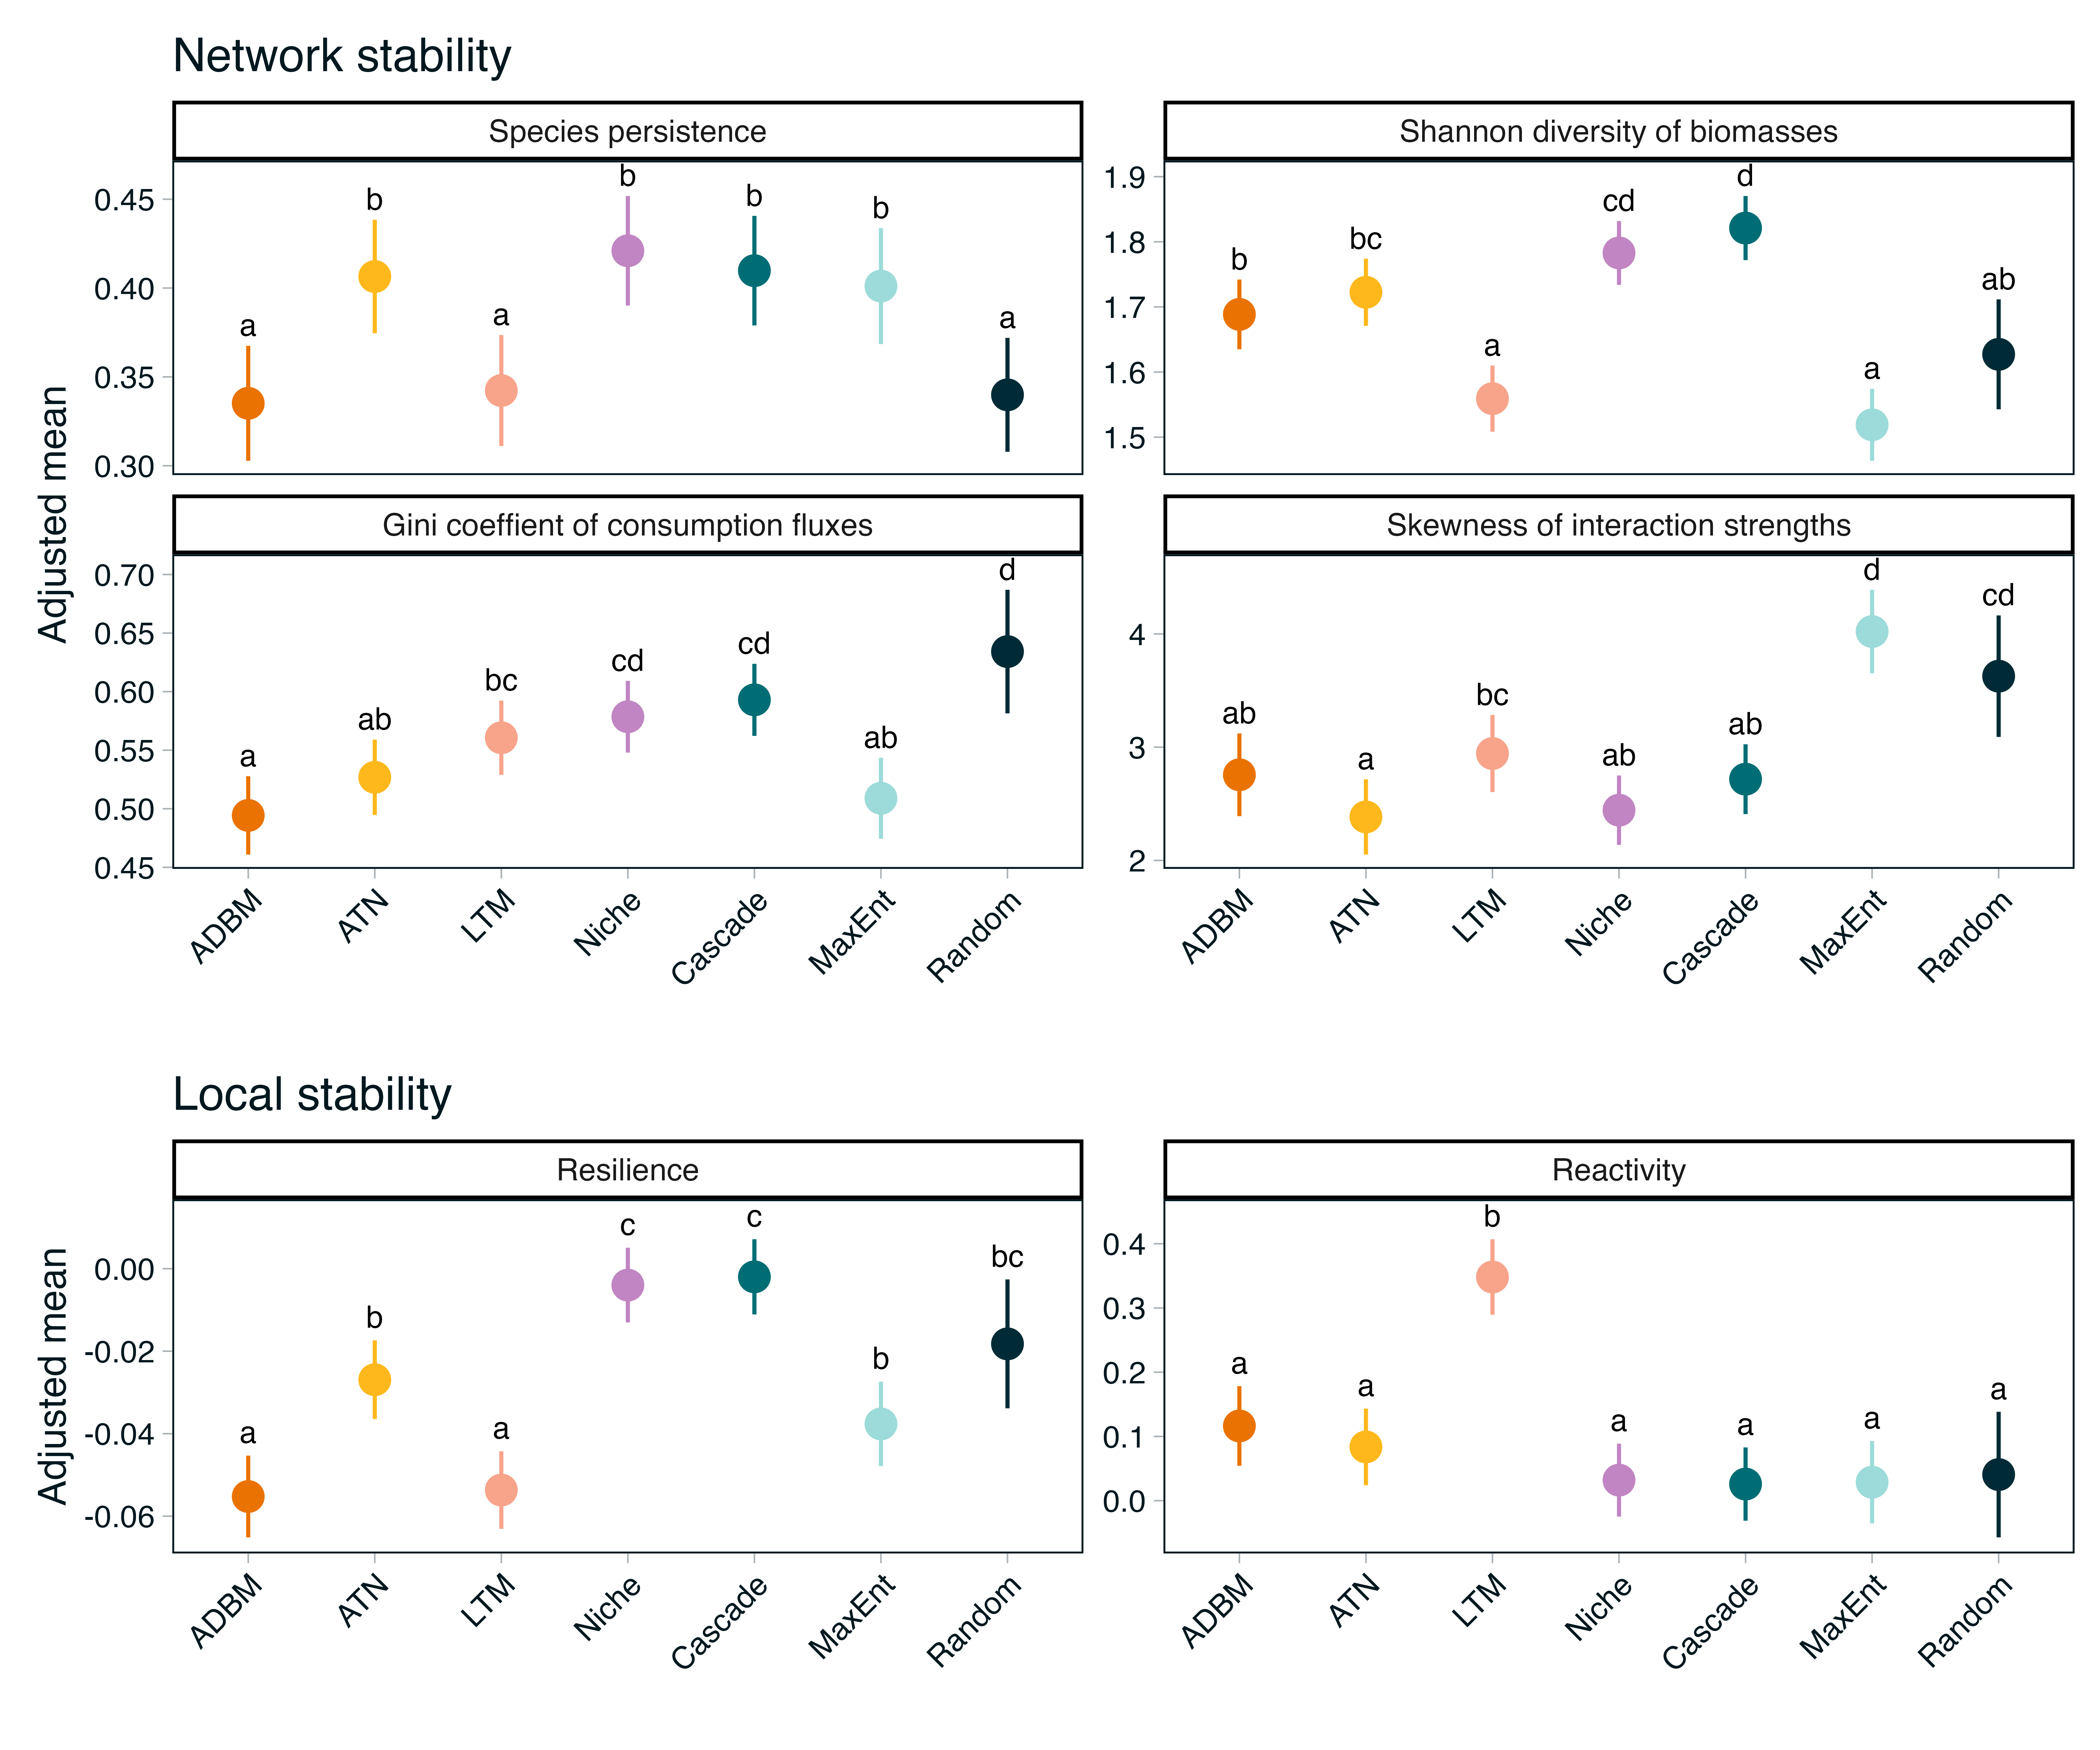
\includegraphics[keepaspectratio]{figures/stability_adjusted_model_means.png}}

}

\caption{\label{fig-emmeans}Network and local stability metrics across
generative food web models. Points are estimated marginal means adjusted
to the mean equilibrium species richness. Bars show 95\% confidence
intervals.}

\end{figure}%

\section{Discussion}\label{discussion}

\subsection{Ecological dynamics constrain food web
structure}\label{ecological-dynamics-constrain-food-web-structure}

One of the clearest results of this study is that ecological dynamics
consistently reduced structural differences among food web
reconstruction frameworks. Networks generated from fundamentally
different structural, statistical, and trait-based assumptions began in
distinct regions of multivariate topology space, yet their realised
counterparts occupied a much narrower region following bioenergetic
simulations. This convergence indicates that ecological dynamics impose
strong constraints on viable food web architecture, regardless of how
the initial network is assembled.

Importantly, this convergence emerged without any opportunity for
networks to rewire. Species interactions remained fixed throughout the
simulations, meaning that all structural change resulted from species
extinctions and the subsequent removal of trophic interactions. The
realised networks therefore represent a filtered subset of the original
architectures rather than newly assembled communities. In this sense,
bioenergetic dynamics act as a selection process on network structure.
Interactions that cannot be maintained under energetic and demographic
constraints are systematically removed, while those compatible with
persistence remain. This interpretation aligns closely with previous
work demonstrating that secondary extinctions reshape food web structure
through dynamic processes that cannot be captured by static robustness
analyses alone (Curtsdotter et al., 2011).

The dominant axis of structural change was associated with reductions in
metrics describing indirect competitive interactions, particularly
exploitative competition (S4). Rather than highlighting these motifs as
special cases, we interpret them as evidence that ecological dynamics
simplify portions of the network where indirect effects are
concentrated. This interpretation is consistent with empirical studies
showing that food webs exhibit conserved local interaction structure
across ecosystems despite substantial differences in species
composition, suggesting that persistent communities occupy a constrained
distribution of these smaller motifs (Stouffer et al., 2007; Stouffer \&
Bascompte, 2010). Our simulations extend this idea by demonstrating that
similar structural organisation can emerge through extinction-driven
filtering, even when networks originate from contrasting generative
assumptions. Moreover, this extinction-driven pruning agrees with the
observation that stable food webs are enriched for interaction
configurations that persist under ecological dynamics, whereas
structurally unstable configurations are selectively removed (Borrelli,
2015).

The behaviour of the Random networks further illustrates the existence
of a constrained structural domain for persistence. Randomly assembled
networks were the least likely to reach equilibrium, particularly as
species richness increased, yet those that did survive underwent
relatively little structural reorganisation. Rather than converging
through extensive pruning, these surviving networks appear to have been
generated close to a dynamically feasible region of topology space by
chance. This result echoes classic stability theory, which predicts that
unconstrained random interaction matrices are overwhelmingly unstable
unless they possess particular structural properties (Allesina \& Tang,
2012; May, 1974). Ecologically informed reconstruction models do not
guarantee persistence, but they substantially increase the probability
of generating networks within this feasible region because their
assembly rules embed ecological constraints absent from purely random
topology (Dunne et al., 2002).

Together, these results suggest that convergence in topology is not
evidence that generative models are interchangeable. Instead, ecological
dynamics compress a diverse set of initial architectures into a narrower
subset of structures compatible with persistence. The important question
therefore becomes whether this shared realised topology also produces
shared ecological dynamics, or whether the assumptions embedded in the
reconstruction framework continue to influence stability despite
structural convergence.

\subsection{Structural convergence does not imply dynamical
equivalence}\label{structural-convergence-does-not-imply-dynamical-equivalence}

Although ecological dynamics drove networks towards a shared region of
topology space, this convergence did not produce equivalent predictions
of community stability. Instead, we observed a clear separation between
coarse dynamic properties, which were largely explained by realised
species richness, and local dynamical properties, which remained
strongly dependent on the original reconstruction framework. Structural
convergence therefore represents only one dimension of ecological
similarity; the dynamical consequences of those structures retain a
signature of how the network was assembled.

This distinction is most apparent when comparing network-level and local
stability metrics. Shannon diversity of biomasses, interaction strength
skewness, species persistence, and the Gini coefficient of consumption
fluxes were explained predominantly by equilibrium richness rather than
model identity. This agrees with longstanding ecological theory showing
that many aggregate properties of communities emerge from biodiversity
itself through biomass partitioning, portfolio effects, and the
distribution of energy across trophic levels (Loreau \& Mazancourt,
2013; Yodzis, 1981). Once ecological dynamics had removed species and
reduced networks to similar realised sizes, these macroscopic properties
became remarkably insensitive to the initial reconstruction framework.

Local stability, however, behaves differently. Reactivity was explained
almost entirely by the generative model, while resilience remained
strongly influenced by model identity even after accounting for realised
richness. These metrics quantify how perturbations propagate through
communities rather than simply whether communities persist, making them
inherently sensitive to the organisation of interaction strengths within
the Jacobian matrix (Neubert \& Caswell, 1997; Tang et al., 2014). Two
networks with similar connectance, trophic structure, and species
richness can therefore exhibit fundamentally different transient
responses if the underlying energetic constraints that generated their
interactions differ.

The contrast between structural and trait-based models illustrates this
point. Niche and Cascade networks consistently reached equilibrium, but
this should not be interpreted as evidence that they provide the most
biologically realistic representation of ecological persistence. Rather,
these models inherit body masses only after network construction through
a fixed predator-prey mass ratio, meaning that energetic structure is
imposed \emph{post hoc} to satisfy the assumptions of the bioenergetic
model (Delmas et al., 2017). In contrast, ADBM, ATN, and latent trait
networks propagate body mass distributions directly from the
reconstruction process into the dynamical model. The resulting
interaction strengths, attack rates, handling times, and metabolic rates
remain coupled through the biological assumptions embedded in each
framework (Brose et al., 2006; Petchey et al., 2008; Schneider et al.,
2016).

This difference helps explain the apparent paradox in our results.
Trait-based models often supported fewer persistent species than
structural models, yet they generated markedly different resilience and
reactivity profiles. In particular, latent trait networks combined
relatively high resilience with the strongest transient amplification of
perturbations, while ADBM networks recovered rapidly despite lower
overall persistence. This decoupling of asymptotic stability from
transient dynamics has been recognised as a defining property of complex
ecological communities where interaction strengths are structured rather
than random (Neubert \& Caswell, 1997; Tang et al., 2014). Consequently,
reproducing global food web topology is not sufficient for reproducing
ecological dynamics.

Our results suggest that structural convergence should not be
interpreted as evidence that reconstruction frameworks become
interchangeable after ecological dynamics. Instead, extinction-driven
filtering removes many topological differences while preserving
historically contingent differences in how energy flows through the
community. The realised network may look similar, but its response to
perturbation still reflects the assumptions embedded in the model used
to generate it.

\subsection{What makes a good food web
model?}\label{what-makes-a-good-food-web-model}

The Niche model transformed food web ecology by demonstrating that
simple assembly rules can reproduce the large-scale architecture of
empirical trophic networks (Williams \& Martinez, 2000). Since then,
structural generative models have become the default starting point for
studies of robustness, extinction cascades, and ecosystem stability
(Allesina \& Tang, 2012; Curtsdotter et al., 2011). Our results do not
challenge the value of these models for describing food web topology.
Instead, they demonstrate that reproducing network structure is not
equivalent to reproducing ecological dynamics.

The central implication of this study is that food web reconstruction
frameworks should be viewed as an embedding of assumptions rather than
interchangeable Null models. Each reconstruction framework encodes
assumptions about the processes that generate trophic interactions,
whether these assumptions arise from niche ordering, statistical
constraints, body size scaling, or optimal foraging. Those assumptions
influence the interaction strengths, energetic organisation, and
transient dynamics that emerge once networks are embedded within a
common dynamical framework. Ecological dynamics subsequently filter
these initial structures towards a shared region of viable topology, but
they do not erase the signature of how those networks were constructed.

This distinction helps reconcile an apparent tension in the food web
literature. Structural models have proven remarkably successful at
reproducing global network statistics across ecosystems, while
mechanistic models have been developed to explain the biological
processes that generate those same interactions (Banville et al., 2023;
Brose et al., 2006; Petchey et al., 2008). Our results suggest that
these approaches answer different ecological questions rather than
competing to identify a single `best' food web model. For questions
concerning broad topological organisation, biodiversity patterns, or
realised species richness, structural and statistical models may provide
appropriate and computationally efficient approximations. In contrast,
questions concerning transient dynamics, perturbation responses,
resilience, or extinction cascades require reconstruction frameworks
that preserve the biological constraints governing interaction strengths
and energy flow (Delmas et al., 2017; Poisot et al., 2016; Schneider et
al., 2016).

More broadly, these findings support a shift in how food web
reconstruction is interpreted. Rather than asking whether one generative
model best represents ecological communities, we should ask whether the
assumptions embedded within a reconstruction framework are appropriate
for the ecological inference being made. As ecological networks are
increasingly reconstructed across space, time, and future environmental
scenarios (Strydom et al., 2021; Strydom, Dunhill, et al., 2026),
explicitly matching reconstruction models to inferential goals will
become as important as matching dynamical models to ecological
processes.

Ultimately, not everything is a niche model. Different reconstruction
frameworks can converge on similar realised network architectures while
retaining fundamentally different predictions about how ecological
communities respond to perturbation. The choice of generative model is
therefore not simply a technical decision about network construction. It
is an ecological hypothesis about how communities are assembled and how
they persist.

\section*{References}\label{references}
\addcontentsline{toc}{section}{References}

\protect\phantomsection\label{refs}
\begin{CSLReferences}{1}{0}
\bibitem[\citeproctext]{ref-adams2009}
Adams, D. C., \& Collyer, M. L. (2009). A GENERAL FRAMEWORK FOR THE
ANALYSIS OF PHENOTYPIC TRAJECTORIES IN EVOLUTIONARY STUDIES.
\emph{Evolution}, \emph{63}(5), 1143--1154.
\url{https://doi.org/10.1111/j.1558-5646.2009.00649.x}

\bibitem[\citeproctext]{ref-allesina2012}
Allesina, S., \& Tang, S. (2012). Stability criteria for complex
ecosystems. \emph{Nature}, \emph{483}(7388), 205--208.
\url{https://doi.org/10.1038/nature10832}

\bibitem[\citeproctext]{ref-banville2023}
Banville, F., Gravel, D., \& Poisot, T. (2023). What constrains food
webs? A maximum entropy framework for predicting their structure with
minimal biases. \emph{PLOS Computational Biology}, \emph{19}(9),
e1011458. \url{https://doi.org/10.1371/journal.pcbi.1011458}

\bibitem[\citeproctext]{ref-bezanson2017}
Bezanson, J., Edelman, A., Karpinski, S., \& Shah, V. (2017). Julia: A
fresh approach to numerical computing. \emph{SIAM Review}, \emph{59}(1),
65--98. \url{https://doi.org/10.1137/141000671}

\bibitem[\citeproctext]{ref-borrelli2015}
Borrelli, J. J. (2015). Selection against instability: Stable subgraphs
are most frequent in empirical food webs. \emph{Oikos}, \emph{124}(12),
1583--1588. \url{https://doi.org/10.1111/oik.02176}

\bibitem[\citeproctext]{ref-brose2006}
Brose, U., Jonsson, T., Berlow, E. L., Warren, P., Banasek-Richter, C.,
Bersier, L.-F., Blanchard, J. L., Brey, T., Carpenter, S. R.,
Blandenier, M.-F. C., Cushing, L., Dawah, H. A., Dell, T., Edwards, F.,
Harper-Smith, S., Jacob, U., Ledger, M. E., Martinez, N. D., Memmott,
J., \ldots{} Cohen, J. E. (2006). Consumer{\textendash}resource
body-size relationships in natural food webs. \emph{Ecology},
\emph{87}(10), 2411--2417.
https://doi.org/\url{https://doi.org/10.1890/0012-9658(2006)87\%5B2411:CBRINF\%5D2.0.CO;2}

\bibitem[\citeproctext]{ref-cohen1990}
Cohen, J. E., Briand, F., \& Newman, C. (1990). \emph{Community food
webs: Data and theory}. Springer-Verlag.
\url{https://www.springer.com/gp/book/9783642837869}

\bibitem[\citeproctext]{ref-curtsdotter2011}
Curtsdotter, A., Binzer, A., Brose, U., De Castro, F., Ebenman, B.,
Eklöf, A., Riede, J. O., Thierry, A., \& Rall, B. C. (2011). Robustness
to secondary extinctions: Comparing trait-based sequential deletions in
static and dynamic food webs. \emph{Basic and Applied Ecology},
\emph{12}(7), 571--580. \url{https://doi.org/10.1016/j.baae.2011.09.008}

\bibitem[\citeproctext]{ref-delmas2017}
Delmas, E., Brose, U., Gravel, D., Stouffer, D. B., \& Poisot, T.
(2017). Simulations of biomass dynamics in community food webs.
\emph{Methods in Ecology and Evolution}, \emph{8}(7), 881--886.
\url{https://doi.org/10.1111/2041-210X.12713}

\bibitem[\citeproctext]{ref-delmas2020}
Delmas, E., Stouffer, D. B., \& Poisot, T. (n.d.). \emph{Food web
structure alters ecological communities top-heaviness with little effect
on the biodiversity-functioning relationship}.
\url{https://doi.org/10.1101/2020.06.10.144949}

\bibitem[\citeproctext]{ref-dunne2002}
Dunne, J., Williams, R. J., \& Martinez, N. D. (2002). Network structure
and biodiversity loss in food webs: Robustness increases with
connectance. \emph{Ecol. Lett.}, \emph{5}(4), 558--567.

\bibitem[\citeproctext]{ref-lajaaiti2025}
Lajaaiti, I., Bonnici, I., Kéfi, S., Mayall, H., Danet, A., Beckerman,
A. P., Malpas, T., \& Delmas, E. (2025). EcologicalNetworksDynamics.jl:
A julia package to simulate the temporal dynamics of complex ecological
networks. \emph{Methods in Ecology and Evolution}, \emph{16}(3),
520--529. \url{https://doi.org/10.1111/2041-210X.14497}

\bibitem[\citeproctext]{ref-loreau2013}
Loreau, M., \& Mazancourt, C. de. (2013). Biodiversity and ecosystem
stability: A synthesis of underlying mechanisms. \emph{Ecology Letters},
\emph{16}(s1), 106--115. \url{https://doi.org/10.1111/ele.12073}

\bibitem[\citeproctext]{ref-may1974}
May, R. M. (1974). \emph{Stability and complexity in model ecosystems}
(Vol. 1). Princeton University Press.
\url{https://doi.org/10.2307/j.ctvs32rq4}

\bibitem[\citeproctext]{ref-neubert1997}
Neubert, M. G., \& Caswell, H. (1997). Alternatives to resilience for
measuring the responses of ecological systems to perturbations.
\emph{Ecology}, \emph{78}(3), 653--665.
\url{https://doi.org/10.1890/0012-9658(1997)078\%5B0653:ATRFMT\%5D2.0.CO;2}

\bibitem[\citeproctext]{ref-petchey2008}
Petchey, O. L., Beckerman, A. P., Riede, J. O., \& Warren, P. H. (2008).
Size, foraging, and food web structure. \emph{Proceedings of the
National Academy of Sciences}, \emph{105}(11), 4191--4196.
\url{https://doi.org/10.1073/pnas.0710672105}

\bibitem[\citeproctext]{ref-poisot2016}
Poisot, T., Stouffer, D. B., \& Kéfi, S. (2016). Describe, understand
and predict: Why do we need networks in ecology? \emph{Functional
Ecology}, \emph{30}(12), 1878--1882.
\url{https://doi.org/10.1111/1365-2435.12799}

\bibitem[\citeproctext]{ref-RCoreTeam2024}
R Core Team. (2024). \emph{R: A language and environment for statistical
computing}. R Foundation for Statistical Computing.
\url{https://www.R-project.org/}

\bibitem[\citeproctext]{ref-rohr2010}
Rohr, R., Scherer, H., Kehrli, P., Mazza, C., \& Bersier, L.-F. (2010).
Modeling food webs: Exploring unexplained structure using latent traits.
\emph{The American Naturalist}, \emph{176}(2), 170--177.
\url{https://doi.org/10.1086/653667}

\bibitem[\citeproctext]{ref-deruiter1995}
Ruiter, P. C. de, Neutel, A.-M., \& Moore, J. C. (1995). Energetics,
patterns of interaction strengths, and stability in real ecosystems.
\emph{Science}, \emph{269}(5228), 1257--1260.
\url{https://doi.org/10.1126/science.269.5228.1257}

\bibitem[\citeproctext]{ref-schneider2016}
Schneider, F. D., Brose, U., Rall, B. C., \& Guill, C. (2016). Animal
diversity and ecosystem functioning in dynamic food webs. \emph{Nature
Communications}, \emph{7}(1), 12718.
\url{https://doi.org/10.1038/ncomms12718}

\bibitem[\citeproctext]{ref-stouffer2010}
Stouffer, D. B., \& Bascompte, J. (2010). Understanding food-web
persistence from local to global scales. \emph{Ecology Letters},
\emph{13}(2), 154--161.
\url{https://doi.org/10.1111/j.1461-0248.2009.01407.x}

\bibitem[\citeproctext]{ref-stouffer2007}
Stouffer, D. B., Camacho, J., Jiang, W., \& Nunes Amaral, L. A. (2007).
Evidence for the existence of a robust pattern of prey selection in food
webs. \emph{Proceedings of the Royal Society B: Biological Sciences},
\emph{274}(1621), 1931--1940.
\url{https://doi.org/10.1098/rspb.2007.0571}

\bibitem[\citeproctext]{ref-strydom2021}
Strydom, T., Catchen, M. D., Banville, F., Caron, D., Dansereau, G.,
Desjardins-Proulx, P., Forero-Muñoz, N. R., Higino, G., Mercier, B.,
Gonzalez, A., Gravel, D., Pollock, L., \& Poisot, T. (2021). A roadmap
towards predicting species interaction networks (across space and time).
\emph{Philosophical Transactions of the Royal Society B},
\emph{376}(1837). \url{https://doi.org/10.1098/rstb.2021.0063}

\bibitem[\citeproctext]{ref-strydom2026}
Strydom, T., Dunhill, A. M., Dunne, J. A., Poisot, T., \& Beckerman, A.
P. (2026). From metawebs to realised webs: A framework for ecological
network representation under global change. \emph{EcoEvoRxiv}.
\url{https://doi.org/10.32942/X2JW8K}

\bibitem[\citeproctext]{ref-strydom2026b}
Strydom, T., Karapunar, B., Dunne, J. A., Hull, P., Little, C. T. S.,
Pimiento, C., Ridgwell, A., Beckerman, A. P., \& Dunhill, A. M. (2026).
\emph{Are we mapping ecosystems or models? Framework choices dominate
food web topology and extinction inferences}.
\url{https://ecoevorxiv.org/repository/view/13495/}

\bibitem[\citeproctext]{ref-tang2014}
Tang, S., Pawar, S., \& Allesina, S. (2014). Correlation between
interaction strengths drives stability in large ecological networks.
\emph{Ecology Letters}, \emph{17}(9), 1094--1100.
https://doi.org/\url{https://doi.org/10.1111/ele.12312}

\bibitem[\citeproctext]{ref-williams2000}
Williams, R. J., \& Martinez, N. D. (2000). Simple rules yield complex
food webs. \emph{Nature}, \emph{404}(6774), 180--183.
\url{https://doi.org/10.1038/35004572}

\bibitem[\citeproctext]{ref-yodzis1981}
Yodzis, P. (1981). The stability of real ecosystems. \emph{Nature},
\emph{289}(5799), 674--676. \url{https://doi.org/10.1038/289674a0}

\end{CSLReferences}





\end{document}
